%
\begin{wrapfigure}{r}{0.35\textwidth} 
   \vspace{-10pt}
	\centering
	\begin{subfigure}[b]{0.48\linewidth}
		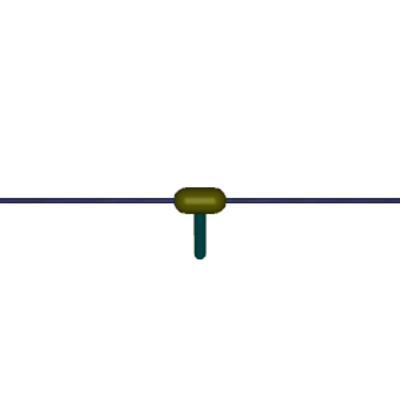
\includegraphics[trim={0 40mm 0 60mm},clip,width=\linewidth]{fig/pendulum.png}
	\subcaption{\small{Cartpole}}
	\end{subfigure}
\hfill
	\begin{subfigure}[b]{0.48\linewidth}
	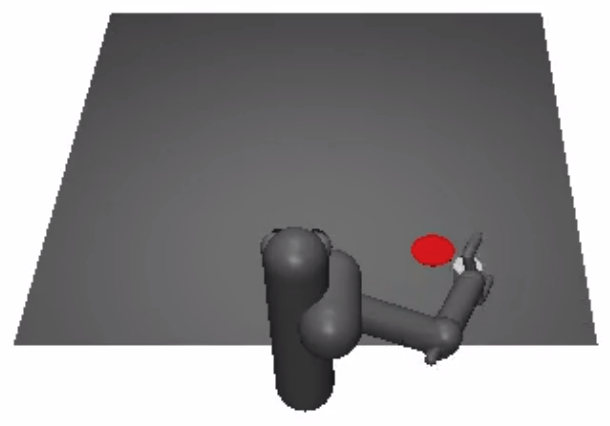
\includegraphics[trim={0 5mm 0 70mm},clip,width=\linewidth]{fig/pusher.png}
	\subcaption{\small{7-dof~Pusher}}
	\end{subfigure}
\\
	\begin{subfigure}[b]{0.48\linewidth}
	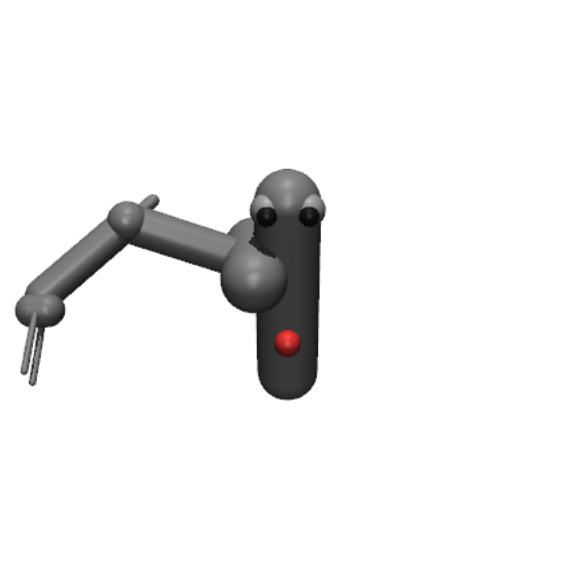
\includegraphics[trim={0 40mm 0 60mm},clip,width=\linewidth]{fig/PR2.png}
	\subcaption{\small{7-dof~Reacher}}
	\end{subfigure}
	\hfill
\begin{subfigure}[b]{0.48\linewidth}
	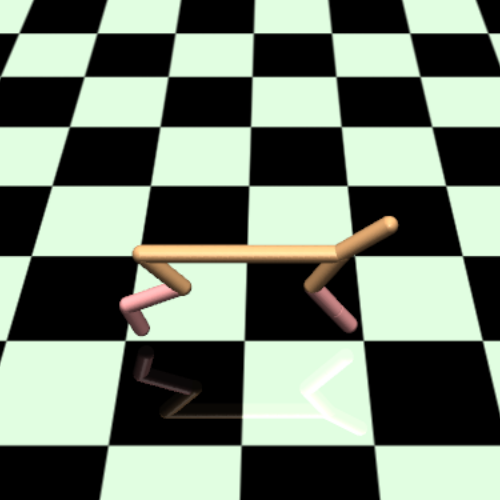
\includegraphics[trim={0 40mm 0 60mm},clip,width=\linewidth]{fig/cheetah.png}
	\subcaption{\small{Half-cheetah}}
	\end{subfigure}
	\caption{Tasks evaluated.}
    \label{fig:results:tasks}
     \vspace{-10pt}
\end{wrapfigure}
%
We now evaluate the performance of our proposed MBRL algorithm called PETS using a deep neural network probabilistic dynamics model.
First, we compare our approach on standard benchmark tasks against state-of-the-art model-free and model-based approaches in \sec{sec:results:comparison-literature}.
Then, in \sec{sec:results:ablation}, we provide a detailed evaluation of the individual design decisions in the model and uncertainty propagation method and analyze their effect on performance. 
Additional considerations of horizon length, action sampling distribution, and stochastic systems are discussed in \app{sec:results:additional}.
The experiment setup is shown in \fig{fig:results:tasks}, and NN architecture details are discussed in the supplementary materials, in \app{sec:results:setting}.
Videos of the experiments, and code for reproducing the experiments can be found at \url{https://sites.google.com/view/drl-in-a-handful-of-trials}.

\subsection{Comparisons to prior reinforcement learning algorithms}
\label{sec:results:comparison-literature}
	%
	\begin{figure}[t]
		\centering
		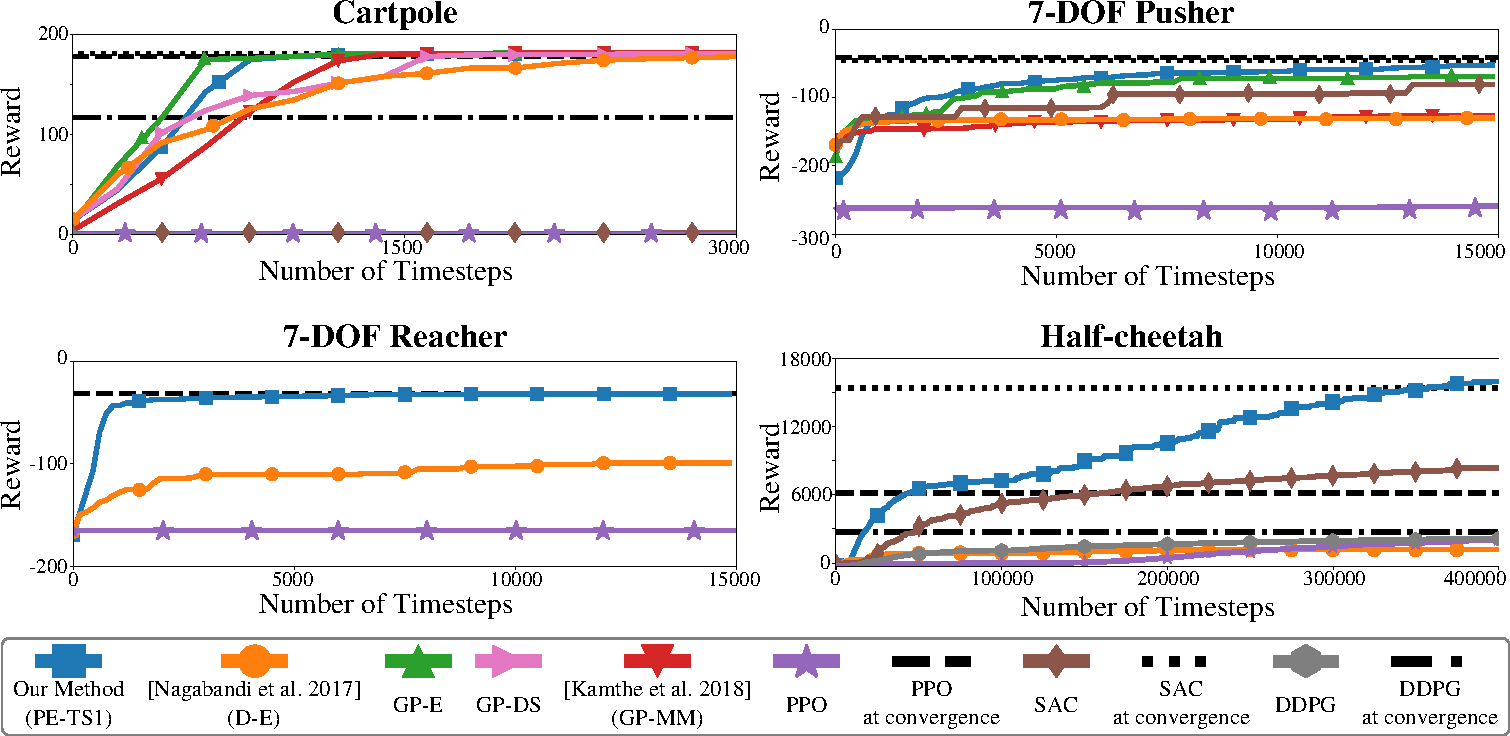
\includegraphics[width=0.98\linewidth]{fig/comparison2.pdf}
		\caption{Learning curves for different tasks and algorithm. 
		For all tasks, our algorithm learns in under 100K time steps or 100 trials.
		With the exception of Cartpole, which is sufficiently low-dimensional to efficiently learn a GP model, our proposed algorithm significantly outperform all other baselines.
For each experiment, one time step equals 0.01 seconds, except Cartpole with 0.02 seconds.
		For visual clarity, we plot the average over 10 experiments of the maximum rewards seen so far.
		}
	    \label{fig:results:comparison-literature}
 	    \vspace{-10pt}
	\end{figure}
	%
	
We compare our \alg{alg:ourmethod} against the following reinforcement learning algorithms for continuous state-action control: 
\begin{itemize}[leftmargin=15pt]
    \item \textbf{Proximal policy optimization (PPO)}: \citep{schulman2017proximal} is a model-free, deep policy-gradient RL algorithm (we used the implementation from \cite{baselines}.)
    \item \textbf{Deep deterministic policy gradient (DDPG)}: \citep{Lillicrap2016} is an off-policy model-free deep actor-critic algorithm (we used the implementation from \cite{baselines}.)
    \item \textbf{Soft actor critic (SAC)}: \citep{Haarnoja2018softUpdated} is a model-free deep actor-critic algorithm, which reports better data-efficiency than DDPG on MuJoCo benchmarks (we obtained authors' data).
\item \textbf{Model-based model-free hybrid (MBMF)}: \citep{Nagabandi2017} is a recent deterministic deep model-based RL algorithm, which we reimplement.
    \item \textbf{Gaussian process dynamics model (GP)}: we compare against three MBRL algorithms based on GPs. GP-E learns a GP model, but only propagate the expectation. GP-DS uses the propagation method DS. GP-MM is the algorithm proposed by~\cite{Kamthe2018} except that we do \textit{not} update the dynamics model after each transition, but only at the end of each trial.
\end{itemize}
%
The results of the comparison are presented in \fig{fig:results:comparison-literature}. 
Our method reaches performance that is similar to the asymptotic performance of the state-of-the-art model-free baseline PPO. 
However, PPO requires several orders of magnitude more samples to reach this point.
We reach PPO's asymptotic performance in fewer than 100 trials on all four tasks, faster than any prior model-free algorithm, and the asymptotic performance substantially exceeds that of the prior MBRL algorithm by \cite{Nagabandi2017}, which corresponds to the deterministic variant of our approach (D-E).
This result highlights the value of uncertainty estimation. 
Whilst the probabilistic baseline GP-MM slightly outperformed our method in cartpole, GP-MM scales cubically in time and quadratically state dimensionality, so was infeasible to run on the remaining higher dimensional tasks.
It is worth noting that model-based deep RL algorithms have typically been considered to be efficient but incapable of achieving similar asymptotic performance as their model-free counterparts. 
Our results demonstrate that a purely model-based deep RL algorithm that only learns a dynamics model, omitting even a parameterized policy, can achieve comparable performance when properly incorporating uncertainty estimation during modeling and planning. 
In the next section, we study which specific design decisions and components of our approach are important for achieving this level of performance.
    
\subsection{Analyzing dynamics modeling and uncertainty propagation}
\label{sec:results:ablation}

    
	\begin{figure}[t]
		\centering
		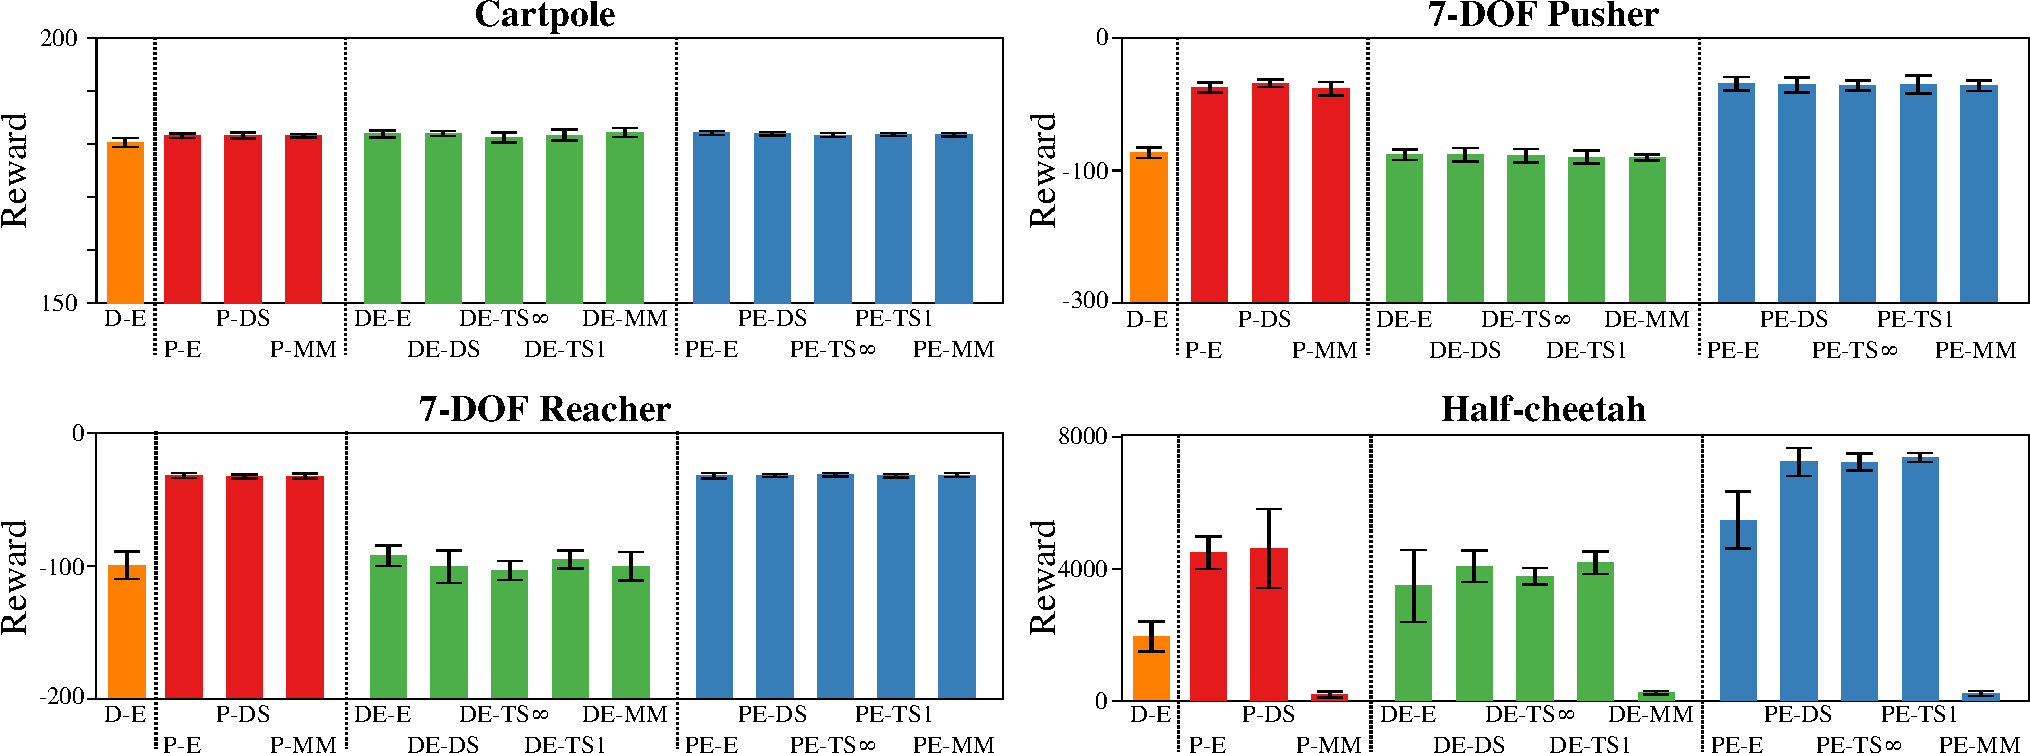
\includegraphics[width=0.98\linewidth]{fig/ablation-bar.pdf}
		\caption{Final performance for different tasks, models, and uncertainty propagation techniques. 
		The model choice seems to be more important than the technique used to propagate the state/action space. 
		Among the models the ranking in terms of performance is: $PE > P > DE > D$.
A linear model comparison can also be seen in \app{app:linear}.
		}
	    \label{fig:results:comparison-ours}
	    	    \vspace{-15pt}
	\end{figure}
    

	In this section, we compare different choices for the dynamics model in \sec{sec:dynamics-models} and uncertainty propagation technique in \sec{sec:approach:propagation}.
    The results in \fig{fig:results:comparison-ours} first show that w.r.t.\ model choice, the model should consider both uncertainty types: the probabilistic ensembles (PE-XX) perform best in all tasks, except cartpole (`X' symbolizes any character).
    Close seconds are the single-probability-type models: probabilistic network (P-XX) and ensembles of deterministic networks (E-XX). 
    Worst is the deterministic network (D-E).
        
	These observations shed some light on the role of uncertainty in MBRL, particularly as it relates to discriminatively trained, expressive parametric models such as NNs. 
	Our results suggest that, the quality of the model and the use of uncertainty at learning time significantly affect the performance of the MBRL algorithms tested, while the use of more advanced uncertainty propagation techniques seem to offers only minor improvements.
	We reconfirm that moment matching (MM) is competitive in low-dimensional tasks (consistent with \citep{Gal2016}), however is not a reliable MBRL choice in higher dimensions, e.g.\ the half cheetah.


The analysis provided in this section summarizes the experiments we conducted to design our algorithm. 
It is worth noting that the individual components of our method -- ensembles, probabilistic networks, and various approximate uncertainty propagation techniques -- have existed in various forms in supervised learning and RL. 
However, as our experiments here and in the previous section show, the particular choice of these components in our algorithm achieves substantially improved results over previous state-of-the-art model-based and model-free methods, experimentally confirming both the importance of uncertainty estimation in MBRL and the potential for MBRL to achieve asymptotic performance that is comparable to the best model-free methods at a fraction of the sample complexity.
